\taughtsession{Lecture}{Describing Language Syntax}{2024-02-16}{14:00}{Jiacheng}{}

\section{Context-Free Grammars}
The linguist Noam Chomsky introduced four classes of formal grammars for describing natural languages:
\begin{itemize}
    \item regular
    \item context-free
    \item context-sensitive
    \item recursively enumerables
\end{itemize}
Of the above listed, two have been found to be useful to describe programming languages:
\begin{itemize}
    \item regular grammars (equivalently, regular expressions) are useful for describing languages' lexical structure
    \item context-free grammars (CFG) for defining their syntax.
\end{itemize}

By far, CGF is the most widely used way to describe a programming language.

\subsection{What is A CFG?}
A CFG is a tuple: $G=(T,N,S,P)$ where:
\begin{itemize}
    \item[$T$] is a finite non-empty set of terminal symbols, which consist of strings in the language (for example \verb|while|), which refer to parts of the text of sentences in the language
    \item[$N$] is a finite non-empty set of non-terminal symbols, disjoint from $T$. These refer to syntactic structures defined by other structures and rules (for example \verb|<exp>|)
    \item[$S$] the start symbol, where $S \in N$
    \item[$P$] is a set of (context-free) productions of the form $A \rightarrow \alpha$ (which reads $A$ produces $\alpha$) where $A \in N$ and $\alpha \in (T \cup N)$
\end{itemize}

\subsection{Example of a CFG}
Taking the CFG as $G_1 = (T, N, S, P)$ where:
\begin{align*}
    T &= \{a, b\}\\
    N &= \{S\}\\
    P &= \{S \rightarrow ab, S \rightarrow aSb\}
\end{align*}
We know that this is a CFG because it has $T$ which is a set of symbols available in the language; $N$ containing the start-state (therefore non-terminal) $S$ and a set of rules of production $P$.\\

To take the CFG $G_2 = (T, N, S, P)$ where:
\begin{align*}
    T &= \{a,b\}\\
    N &= \{S,C\}\\
    P &= \{S \rightarrow \varepsilon, S \rightarrow C, S \rightarrow aSa, s \rightarrow bSb, C \rightarrow a, C \rightarrow b \}
\end{align*}

\subsection{Shorthand Notation}
It's lovely writing the CFGs out in full however this takes up quite a lot of space. So, instead of writing each individual rules of a given non-terminal, we are able to group the alternative right hand sides and separate them using $|$. For example, $G_2$ can be written as follows:
\begin{align*}
    S & \rightarrow \varepsilon | C | aSa | bSb\\
    C & \rightarrow a | b
\end{align*}

\subsection{Symbol Choice Conventions}
As we have seen in the above examples, there is a standard naming conventions for the symbols used:
\begin{itemize}
    \item $a, b, c, \ldots$ for members of $T$ (single terminal symbols)
    \item $A, B, C, \ldots$ for members of $N$ (single non-terminal symbols)
    \item $\ldots, X, Y, Z$ for members of $T \cup N$ (single symbols, terminal or non-terminal)
    \item $w, x, y, z, \ldots$ for members of $T^*$ (strings of terminal symbols)
    \item $\alpha, \beta, \gamma, \ldots$ for members of $(T\cup N)^*$ (mixed strings of terminals and / or non-terminal symbols)
\end{itemize}
Here $a, b, c, \ldots$ refer to letters at the beginning of the alphabet (the set of all symbols) and $w, x, y, z, \ldots$ to letters at the end of the alphabet.

\section{Backus-Naur Form (BNF)}
Backus-Naur Form (BNF) is a popular notation for CFG definitions of real programming languages. BNF uses angle brackets to denote non-terminal symbols, in a similar way to XML tags. For example \verb|<exp>|, \verb|<number>| and \verb|<digit>| are non-terminal; while \verb|+|, \verb|-|, \verb|*|, \verb|/|, \verb|0|, \verb|1|, \ldots{} \verb|9| are terminal symbols. 

\subsection{Syntactic Structures}
Using the above symbols, the syntactic structure for arithmetic expression would be defined by the following productions:
\begin{lstlisting}
    <exp> $\rightarrow$ <exp> + <exp> | <exp> + <exp> | 
             <exp> * <exp> | <exp> / <exp> | (<exp>) | <number>
    
    <number> $\rightarrow$ <digit> | <digit> <number>

    <digit> $\rightarrow$ 0 | 1 | 2 | 3 | 4 | 5 | 6 | 7 | 8 | 9 
\end{lstlisting}
    
In the above example, \verb|<exp>|, \verb|<number>| and \verb|<digit>| are non-terminals while \verb|+|, \verb|-|, \verb|*|, \verb|/|, \verb|0|, \verb|1|, \ldots{} \verb|9| are terminals. 

\subsection{Grammar for a Simple Language}
Below is a complete example of a BNF definition for a simple language:
\begin{lstlisting}
      <program> $\rightarrow$ begin <stmt-list> end
    <stmt-list> $\rightarrow$ <stmt> | <stmt> ; <stmt-list>
         <stmt> $\rightarrow$ <assign>
                   | <input-stmt>
                   | <output-stmt>
       <assign> $\rightarrow$ <ident> := <exp>
          <exp> $\rightarrow$ <ident> | <exp> + <exp>
   <input-stmt> $\rightarrow$ input <ident>
  <output-stmt> $\rightarrow$ output <ident>
        <ident> $\rightarrow$ x | y | z
\end{lstlisting}

\section{Derivations}
We can use a Context-Free Grammar to \textit{derive} strings of terminal symbols. Starting with the start symbol, $S$, we repeatedly apply the production rules until we obtain a string comprising only of terminal symbols, which is called a sentence. This process is called a derivation. Every string of symbols in a derivation is a sentential form. \\

The language defined by a grammar is made up of exactly those sentences that can be derived from it.
\subsection{An Example}
If we consider the grammar $G_2 (T, N, S, P)$ where:
\begin{align*}
    T &= \{a,b\}\\
    N &= \{S,C\}\\
    P &= \{S \rightarrow \varepsilon, S \rightarrow C, S \rightarrow aSa, s \rightarrow bSb, C \rightarrow a, C \rightarrow b \}
\end{align*}
We are able do derive the string $abbba$ for $G_2$ in the following steps:
\begin{enumerate}
    \item We begin with the start symbol $S$
    \item Applying the rule $S \rightarrow aSa$, we replace the $S$ by $aSa$ to obtain the string $aSa$.
    \item Applying the rule $S \rightarrow bSb$ on the new string $aSa$, we replace the $S$ by $bSb$ to obtain the string $abSba$
    \item Applying the rule $S \rightarrow C$, we obtain the string $abCba$
    \item Applying the rule $C \rightarrow b$, we obtain the string $abbba$ of terminal symbols.
\end{enumerate}

\subsection{Notation}
As we can see above, that is quite a long handed approach to righting out a derivation. There is a shorthand way of writing out a derivation as we will see below.\\

If we can get from $\alpha$ to $\beta$ by applying a single application rule, we say $alpha$ immediately derives $\beta$ written
\[\alpha \Rightarrow \beta\]
(note the double line'd arrow used here, not a single line as we have seen above for production rules)\\

We can therefore write the full derivation of $abba$ from $S$ as:
\begin{align*}
    S & \Rightarrow aSa\\
    & \Rightarrow abSba\\
    & \Rightarrow abCba\\
    & \Rightarrow abbba
\end{align*}

\subsection{Full Derivation Example}
We've now seen all the components to derivation, so now we will see a full example. The grammar of our language is as follows:
\begin{lstlisting}
    <program> $\rightarrow$ <stmts>
      <stmts> $\rightarrow$ <stmt> | <stmt> ; <stmts>
       <stmt> $\rightarrow$ <var> = <expr>
        <var> $\rightarrow$ a | b | c | d
       <expr> $\rightarrow$ <term> + <term> | <term> - <term>
       <term> $\rightarrow$ <var> | const
\end{lstlisting}
In the above grammar, \verb|<program>| is the start symbol, making it non-terminal; \verb|<stmt>|, \verb|<stmts>|, \verb|<expr>|, \verb|<term>|, and \verb|<var>| are non-terminals; whereas \verb|a|, \verb|b|, \verb|c|, \verb|d|, \verb|+|, \verb|-| and \verb|const| are terminals. \\

We can derive a single line program:
\begin{center}
    \verb|a = b + const|
\end{center}
from this grammar:
\begin{lstlisting}
    <program> $\Rightarrow$ <stmts>
              $\Rightarrow$ <stmt>
              $\Rightarrow$ <var> = <expr>
              $\Rightarrow$ a = <expr>
              $\Rightarrow$ a = <term> + <term>
              $\Rightarrow$ a = <var> + <term>
              $\Rightarrow$ a = b + <term>
              $\Rightarrow$ a = b + const
\end{lstlisting}
Lines 5 and 6 are in Sentential Form and the final line (ln. 8) is the finished sentence.\\

There is a second example of a derivation in the \verb|lecture06| slides on Moodle.

\subsection{Leftmost \& Rightmost Derivations}
Considering the following grammar for arithmetic expression
\begin{lstlisting}
    <exp> $\rightarrow$ <exp> + <exp> | <exp> * <exp> | x | y | z
\end{lstlisting}
A derivation of the sentence \verb|x + y * z| from this grammar could be:
\begin{lstlisting}
    <exp> $\Rightarrow$ <exp> + <exp>
          $\Rightarrow$ x + <exp>
          $\Rightarrow$ x + <exp> * <exp>
          $\Rightarrow$ x + y * <exp>
          $\Rightarrow$ x + y * z
\end{lstlisting}
Which is known as a \textit{leftmost} derivation because, at each step, the leftmost non-terminal symbol is resolved.\\

It is also possible to have a rightmost derivation:
\begin{lstlisting}
    <exp> $\Rightarrow$ <exp> + <exp>
          $\Rightarrow$ <exp> + <exp> * <exp>
          $\Rightarrow$ <exp> + <exp> * z
          $\Rightarrow$ <exp> + y * z
          $\Rightarrow$ x + y * z
\end{lstlisting}

It is also possible to have a neither left-nor right-most:
\begin{lstlisting}
    <exp> $\Rightarrow$ <exp> + <exp>
          $\Rightarrow$ <exp> + <exp> * <exp>
          $\Rightarrow$ <exp> + y * <exp>
          $\Rightarrow$ x + y * <exp>
          $\Rightarrow$ x + y * z
\end{lstlisting}

\section{Parse Trees}
We are able to illustrate the structure of an the expression given by a derivation as a parse tree.
\begin{figure}[H]
\centering
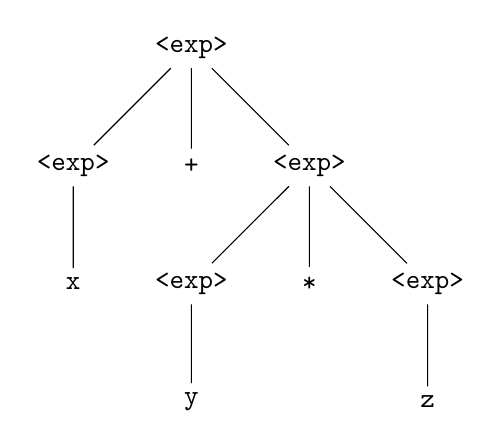
\begin{tikzpicture}[font=\ttfamily]
\node{<exp>}   
    child {node {<exp>}
        child {node {x}}}
    child {node {+}}
    child {node {<exp>}
        child {node {<exp>}
            child {node {y}}}
        child {node{*}}
        child {node {<exp>}
            child {node {z}}}};
\end{tikzpicture}
\caption{Parse Tree for derivation of \texttt{x + y * z}}
\end{figure}

The derivation of \verb|x + y * z| can be seen below
\begin{lstlisting}
    <exp> $\Rightarrow$ <exp> + <exp>
          $\Rightarrow$ x + <exp>
          $\Rightarrow$ x + <exp> * <exp>
          $\Rightarrow$ x + y * <exp>
          $\Rightarrow$ x + y * z
\end{lstlisting}

The internal nodes of the parse tree contin non-terminal symbols whereas leaf nodes contin terminal symbols. \\

It should be noted that for some grammars, the derivation of a given sentence can be different. Meaning they have different parse trees. This will commonly be the case when applying different ordered derivations.